\chapter{\label{ch:3-gb-result}Understanding population structure in Africa using GhostBuster}

\minitoc

\section{Chapter overview}

In this chapter, we apply GhostBuster to real genetic data from the Human Genome Diversity Project (HGDP) and the $1{,}000$ Genomes Project ($1{,}000$ GP) to better understand the evolutionary history of humans in Africa. The chapter is divided into two main sections based on the type of event we discuss.

In Section \ref{sec:ch3-gb-bta}, we find evidence for back-to-Africa migration, which introduced Eurasian ancestry into Africa. We estimate this event occurred approximately $5{,}000$ to $15{,}000$ years ago, contributing up to 8\% to the genetic makeup of modern-day sub-Saharan Africans. In this section, we characterize and validate the admixture event, including dating the event, identifying potential source populations, and performing independent validations such as correlating Neanderthal ancestry with Eurasian ancestry in Africa and examining mutational enrichment profiles conditioned on local ancestry. Additionally, we find signatures of adaptive introgression resulting from this back-to-Africa gene flow.

In Section \ref{sec:ch3-gb-deep}, we explore and seek to understand the complex population structure in Africa before the Out of Africa event. Consistent with existing literature, we find evidence for deep population structure in Africa, with up to four ancestral components present more than $100{,}000$ years ago. These components mixed and merged in varying proportions to form present-day African populations. We also find that some of these components show excess affinity towards Neanderthals and Denisovans and exhibit differences in PRDM9 allele types. Finally, we use the inferred local ancestry to assess PGS portability for different African components, finding better PGS portability for components that contributed extensively to the Out of Africa population.  

 
\section{Back to Africa migration}
\label{sec:ch3-gb-bta}

Present-day Africans constitute a significant portion of the global population, with approximately 1.28 billion individuals.
%
This large demography also exhibits a high level of genetic diversity, which is greater than any other human population.
%
Indeed, Africans exhibit nearly twice the average nucleotide diversity compared to their Asian and European counterparts \cite{yu2002larger}. 
%
Despite this remarkable genetic richness, our understanding of the historical narratives and evolutionary trajectories of African populations remains limited. 


Migrations from Eurasia into Africa have been identified before. 
%
In fact, North African groups such as the Mozabites, Moroccans, Tunisians, and Egyptians have a significant portion of their ancestry derived from European or Middle Eastern populations, with evidence of recent admixture occurring 500-1000 years ago \cite{price2009sensitive, hellenthal2014genetic, salter2019fine}. 
%
One of the primary barriers to migration into Africa is the vast Sahara Desert, which would have impacted migrations from Eurasia into sub-Saharan Africa.
%
However, it is well known that the Sahara underwent periodic climate cycles due to changes in Earth's orbit, transitioning between arid and humid phases. 
%
The humid phase, often referred to as the ``Green Sahara'' period, could have made migrations into and out of Africa more feasible. The last Green Sahara period occurred approximately $5{,}000$ to $11{,}000$ years ago \cite{tierney2017rainfall, larrasoana2013dynamics}.

One of the first work to identify potential Eurasian ancestry in sub-Saharan Africans was conducted by Pickrell et al. \cite{pickrell2012genetic, pickrell2014ancient}.
%
They used ALDER \cite{loh2013inferring}, a method to identify and date admixture signal through LD decay curves (as described in section \ref{sec:ch1-gb-survey}) and found evidence for west Eurasian ancestry in south and east African populations, but not in West or central Africans. 
%
They estimated the proportions of west Eurasian ancestry to be up to 14\% in south African populations and up to 50\% in east African populations. These admixture events were dated to approximately 900–$1{,}800$ years ago in south Africa and $2{,}700$–$3{,}300$ years ago in east Africa. 
%
Additionally, they found the Eurasian ancestry in south Africa and east Africa to be shared and therefore theorized the most likely explanation of Eurasian ancestry in south Africa to be from east Africa.
%
While the study convincingly argued for a ``back to Africa'' migration event, the method's limited statistical power and reliance on reference populations may have hindered the detection of similar events in other African populations. 
%
These populations might have experienced smaller proportions of Eurasian ancestry or older admixture events, which were beyond the resolution of the study.

In another study, Llorente et al. \cite{llorente2015ancient} sequenced an ancient individual from the Mota caves in Ethiopia, who lived approximately 4,500 years ago. %% cite the erratum
%
This ancient DNA sample provided more direct evidence for Eurasian ancestry in African populations, as it was considered to predate the back to Africa event and thus served as a reference population without any Eurasian ancestry.
%
Using the Mota individual as a reference, the study found 4 to 7\% higher west Eurasian ancestry in east Africa, along with a much broader geographic impact of the backflow, extending to west and south Africa. 
%
They detected 7\% and 6\% Eurasian ancestry in present-day Yoruba and Mbuti individuals, respectively, populations that previously showed no signs of Eurasian ancestry and were considered ideal references for African populations. remove this sign!! %% caution!!
%
Overall, The ancient DNA provided further evidence for the backflow event affecting a wider range of African populations. However, it relied on the assumption that the ancient sample had no Eurasian ancestry, which could lead to an underestimation of Eurasian ancestry in modern African samples.
%
In fact, as we demonstrate in a later section, using our method, which does not rely on a reference population, we found some Eurasian ancestry in the Mota individual as well.

Several studies have identified small amounts of Neanderthal ancestry in African individuals, suggesting a back to Africa migration as a plausible explanation \cite{chen2020identifying,vernot2016excavating}. 
%
Chen et al. \cite{chen2020identifying} developed a novel method called IBDmix to detect introgressed Neanderthal sequences in African individuals. They discovered that modern-day Africans carry between 16.4 and 18 megabases (Mb) of Neanderthal sequence per individual, which is roughly one-third of the Neanderthal sequence found in modern-day non-Africans. 
%
Interestingly, 94\% of the Neanderthal sequences identified in African samples were shared with non-Africans, with a significantly higher overlap observed with Neanderthal sequences found in Europeans compared to East Asians.
%
The study's findings align with a model involving an ancient migration of humans to Neanderthal regions, followed by a more recent back migration to Africa. This model closely fits the observed genetic patterns.
%
Overall, the study provides independent validation of a backflow event into Africa, though it does not have the resolution to precisely characterize the proportions and timings of this event.

Finally, ancient DNA from North Africa has revealed significant migrations from the Middle East and Europe into the African continent \cite{van2018pleistocene, fregel2018ancient, simoes2023northwest}.
%
The Taforalt individual, sequenced from eastern Morocco and dated to $15{,}000$ years ago, exhibited genetic composition that was two-thirds similar to Middle Eastern hunter-gatherers and one-third similar to sub-Saharan Africans \cite{van2018pleistocene}.
%
Recent studies have uncovered additional ancient DNA in North Africa, indicating not only migrants from the Middle East but also European Neolithic farmers who introduced new lifestyles to North Africa between $7{,}000$ and $9{,}000$ years ago \cite{fregel2018ancient, simoes2023northwest}. 
%
These migrations from the Middle East and Europe likely influenced the genetics of populations throughout the rest of Africa, affecting the genetic makeup of present-day samples.


\subsection{1-8\% Eurasian ancestry in sub-Saharan African individuals}

We analyzed 17 sub-Saharan African groups across the human genome diversity project (HGDP), the 1,000 Genomes Project (1,000 GP) and Simon's genome diversity project (SGDP) and found upto 8\% Eurasian ancestry in these African populations. The groups we analyzed are listed in table \ref{tab:african_populations}a. Additionally, we also analyzed a five ancient samples in Africa, including a 8,000 year old sample from Shum Laka in Cameroon \cite{lipson2020ancient}, 2,000 and 400 year old samples from Ballito Bay, Eland Cave and Newcastle in South Africa \cite{schlebusch2017southern} and 4,500 year old sample from Mota cave in Ethiopia \cite{llorente2015ancient} (see table \ref{tab:african_populations}b). A map with all modern and ancient samples analyzed is shown in Figure \ref{fig:gb-afr-samples-map}.


\begin{table}[h!]
\centering
\begin{subtable}{\textwidth}
\centering
\resizebox{\textwidth}{!}{
\begin{tabular}{|l|l|l|c|}
\hline
\textbf{Population} & \textbf{Dataset} & \textbf{Location} & \textbf{Samples} \\ \hline
Esan & $1{,}000$GP & Nigeria & 20 \\ \hline
Gambian & $1{,}000$GP & Gambia & 20 \\ \hline
Luhya & $1{,}000$GP & Kenya & 20 \\ \hline
Mende & $1{,}000$GP & Sierra Leone & 20 \\ \hline
Biaka & HGDP & Central African Republic & 22 \\ \hline
Mandenka & HGDP & Senegal & 21 \\ \hline
Mbuti & HGDP & Democratic Republic of Congo & 12 \\ \hline
San & HGDP & Namibia and South Africa & 6 \\ \hline
Yoruba & HGDP & Nigeria & 21 \\ \hline
Bantu Kenya & HGDP & Kenya & 11 \\ \hline
Bantu SouthAfrica & HGDP & Botswana or Namibia & 8 \\ \hline
Somali & SGDP & Kenya & 2 \\ \hline
Luo & SGDP & Kenya & 2 \\ \hline
Masai & SGDP & Kenya & 2 \\ \hline
Ju Hoan North & SGDP & Namibia & 4 \\ \hline
Dinka & SGDP & Sudan & 3 \\ \hline
Khomani San & SGDP & South Africa & 2 \\ \hline
\multicolumn{3}{|l|}{\textbf{Total}} & \textbf{196} \\ \hline
\end{tabular}}
\caption{}
\label{tab:african_populations_1}
\end{subtable}

\vspace{1cm} % Adjust space between tables as needed

\begin{subtable}{\textwidth}
\centering
\resizebox{\textwidth}{!}{
\begin{tabular}{|l|l|l|l|c|}
\hline
\textbf{ID} & \textbf{Publication} & \textbf{Location} & \textbf{Coverage} & \textbf{Age} \\ \hline
I10871 & Lipson et al. \cite{lipson2020ancient} & Shum Laka, Cameroon & 18.51 & 7890 \\ \hline
new001 & Schlebusch et al. \cite{schlebusch2017southern} & Newcastle, South Africa & 11.073 & 418 \\ \hline
ela001 & Schlebusch et al. \cite{schlebusch2017southern} & Eland Cave, South Africa & 10.52 & 493 \\ \hline
baa001 & Schlebusch et al. \cite{schlebusch2017southern} & Ballito Bay A, South Africa & 12.93 & 1909 \\ \hline
I5950 & Llorente et al. \cite{llorente2015ancient} & Mota cave, Ethiopia  & 11.28 & 4472 \\ \hline
\multicolumn{4}{|l|}{\textbf{Total}} & \textbf{5} \\ \hline
\end{tabular}}
\caption{}
\label{tab:african_populations_2}
\end{subtable}

\caption{\textbf{Sub-Saharan African populations analyzed.} (a) Modern samples and, (b) Ancient samples}
\label{tab:african_populations}
\end{table}

\begin{figure}[h!]
    \centering
    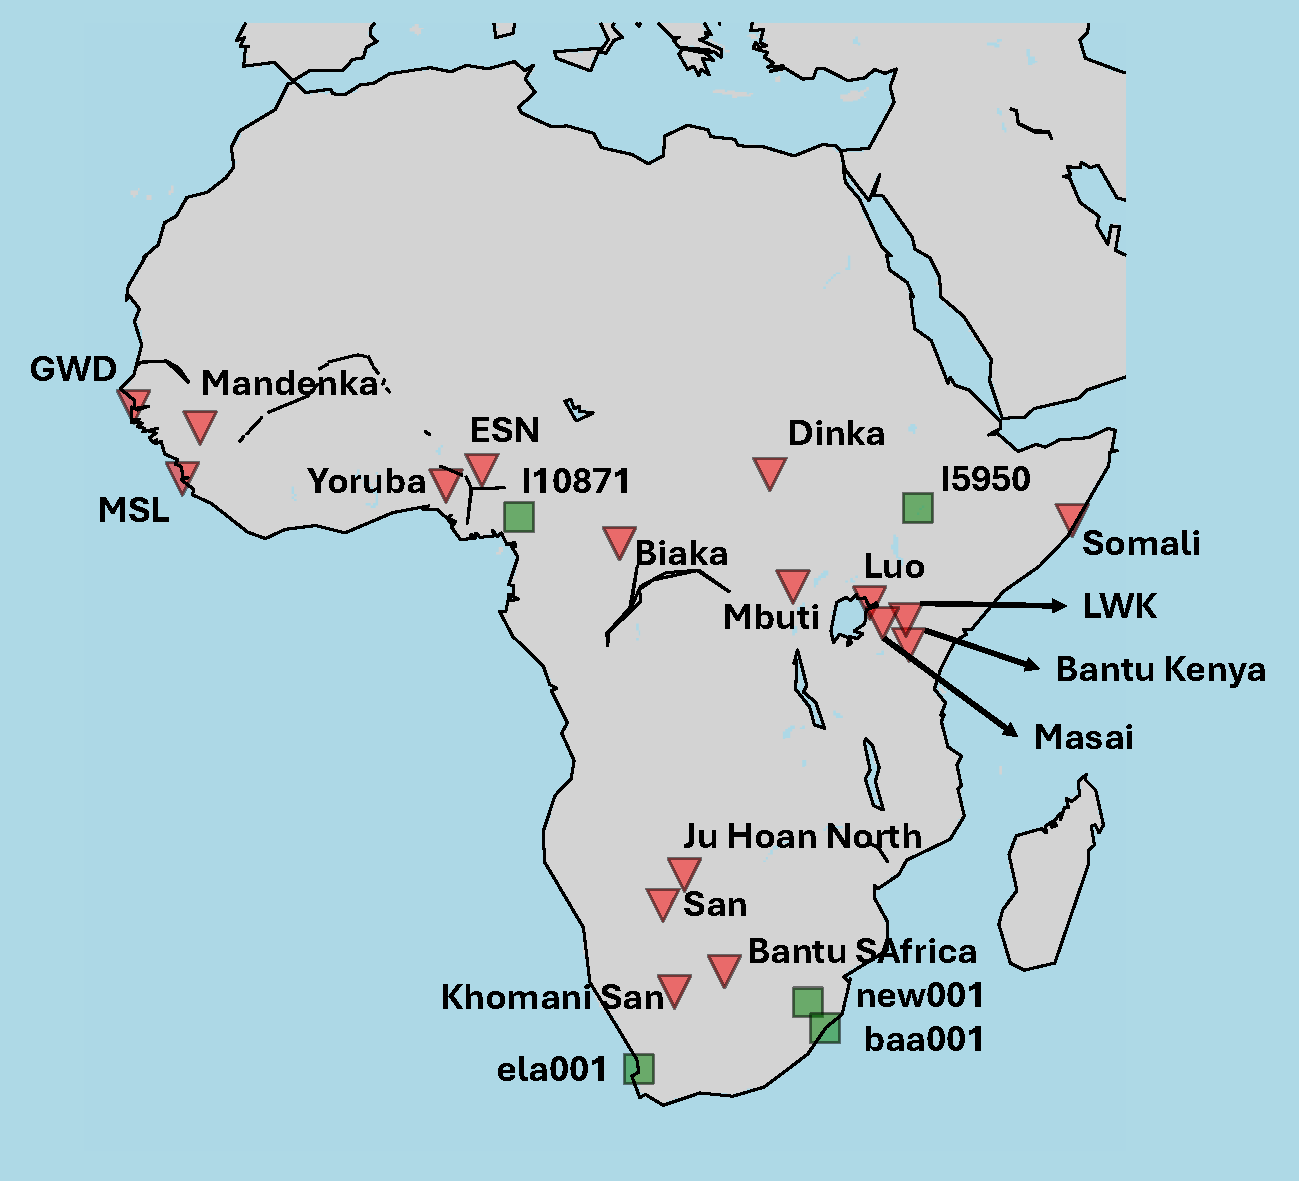
\includegraphics[width=0.75\textwidth]{figures/thesis_afr_samples.pdf}
    \caption{\textbf{Map of the African samples analyzed.} Red inverted triangles correspond to modern samples in HGDP, 1,000GP and SGDP, and green squares 5 ancient African samples.}
    \label{fig:gb-afr-samples-map}
\end{figure}


%% better population labeling
%% add SGDP ?
%% add ancients? 


% how did we run the method? 
%% 1. Combined nfe, eas and sas group and called them Eurasians.
%% 2. Epochs = 0 to 50,000 years (looking at more recent event)
%% 3. Fixed the coalescene rates based on coalescene rates for Eurasian and African segments, varied the proportions and admixture time
%% 4. Fit each African group seperately.

% main result
%% 1. We found 1-8\% Eurasian ancestry across the groups we analyzed
%% 2. Highest in ..., lowest in ... 
%% 3. Among ancient samples, Mota had .., whereas balito boy didn't have any. 
%% 4. We replicated the finding in SGDP, and found the local ancestry inferred for the same samples to be highly correlated.
%% 5. Ablations: hmm vs no hmm, changing epoch boundries
%% 6. PCA visualization

\subsection{Dating the admixture event}

%% LD-decay curves
%% Showing it was continous migration? plot the coal. time vs. segment length

\subsection{Eurasian ancestry explains the Neanderthal ancestry in Africa}

% cite: The Neanderthal ancestry in modern Africans can be explained by back migration from an ancestral European- like source into Africa (72), a scenario which is supported by other studies that found Neanderthal ancestry proportions to correlate with Eurasian ancestry proportions (21,32,73,74). (Hollfelder et al. 2021)

%% Corr. in proportion
%% Enrichment in local ancestry

\subsection{Mutational profiles validate Eurasian segments in Africa}

%% TCC-TTC
%% weak-strong

\subsection{Identifying the source groups}

%% Coal. rate with moderns
%% Coal. rate with ancients

\subsection{Signatures of positive selection} 

%% Assuming a simple piecewise-constant model, we infer that the rate of TCC → TTC mutations increased dramatically  ∼ 15,000 years ago and decreased again  ∼ 2000 years ago. This time-range is consistent with results showing this signal in a pair of prehistoric European samples from 7000 and 8000 years ago, respectively (Mathieson and Reich, 2016). We hypothesize that this mutation pulse may have been caused by a mutator allele that drifted up in frequency starting 15,000 years ago, but that is now rare or absent from present day populations. (see: https://www.ncbi.nlm.nih.gov/pmc/articles/PMC5435464/)


\section{Deep population structure in Africa}
\label{sec:ch3-gb-deep}

% Africa's importance in human population genetics
Africa is widely recognized as the cradle of modern humans. 
%
Fossil evidence of Homo sapiens dating back $300{,}000$ years \cite{day1969early,hublin2017new}, along with population genetics data showing high genetic diversity and the presence of some of the deepest population splits, supports this view.
%
Despite its significance in understanding human origins, the genetic history of Africa during the middle ($781{,}000$ to $126{,}000$ years ago) and late Pleistocene ($126{,}000$ to $11{,}700$ years ago) remains poorly understood. 
%
This is due to several challenges, including the lack of ancient DNA from the region, as the hot and humid climate hinders its preservation. And, recent demographic changes, such as back-to-Africa migrations (as discussed in section \ref{sec:ch3-gb-bta}), the Bantu expansion \cite{tishkoff2009genetic}, and European colonization which obscure the ancient signals when analyzing modern samples.

The population structure in Africa prior to the Out of Africa event has been a topic of considerable debate, with compelling evidence supporting the existence of structured populations even before humans expanded out of Africa.
%
Scerri et al. \cite{scerri2019beyond} argue that fossil data from Africa do not reflect contemporary humans emerging progressively in a single region. Instead, these fossils suggest that humans appeared at different times and in various combinations, exhibiting diverse ancestral features. This view is bolstered by evidence of polycentric origins of modern cognition and paleo-climatic models indicating periodic climate fluctuations.
%
The structured African metapopulation model proposed by Scerri et al. challenges the simple tree-like model of human evolution. This model suggests that ancient populations could coalesce, split, experience gene flow, or go extinct over time. Scerri et al. found that the structured metapopulation model, also referred to as the ``population fragmentation and coalescence model'', better explains the genetic and archaeological data compared to a simple panmixia model, which assumes a single, interbreeding population.

There has also been considerable research showing evidence for unsampled or `ghost' archaic hominids in Africa \cite{ragsdale2019models,hammer2011genetic,lorente2019whole,durvasula2020recovering}. For instance, Durvasula et al. employed the conditional site frequency spectrum (CSFS) to identify an archaic component in West Africans which diverged from modern humans more than $700{,}000$ years ago and contributed up to 19\% to the genetic makeup of present-day West African populations recently. Although its claims, archaic introgression in Africa is still debated as methods fail to account for the possibly complex population structure in Africa.
%
Despite these debates, African populations exhibit far more long genetic branches than non-African populations, with an average of $42{,}434$ mutations in Africans compared to $7{,}012$ in non-Africans. This suggests more complex population dynamics, either due to archaic introgression or isolation by distance \cite{speidel2019method}.

Hollfelder et al. \cite{hollfelder2021deep} and Ragsdale et al. \cite{ragsdale2023weakly} argue that the model of archaic admixture in Africa does not fully explain the genetic diversity of present-day African populations. Ragsdale et al. applied a maximum likelihood framework to infer demographic parameters that best explain the one- and two-locus statistics for various African groups. They found that the ``population fragmentation and coalescence model'' \cite{scerri2019beyond} consistently outperformed other models, including those involving archaic admixture in Africa. The proposed model by Ragsdale et al. describes a weakly structured stem, with three co-existing stem populations more than $100{,}000$ years ago. These populations underwent migration among themselves and eventually merged in different proportions to form present-day African populations. The model proposed better fits the archaeological data around that time but still suffers from model mis-specification as it constrains the possibility of models while inferring the demographic parameters.

Ancient DNA in Africa is scarce due to poor preservation in hot and humid conditions, but there are a few samples spanning the past $18{,}000$ years. Lipson et al. \cite{lipson2022ancient} argue that analyzing these ancient samples helps reduce confounding factors from more recent events such as back-to-Africa migrations, the Bantu expansion, and European colonization. By studying the ancient DNA of 31 samples, they aimed to understand the population structure of hunter-gatherers in central and southern Africa, which represent some of the deepest splits in modern human lineages. Using supervised PCA, the researchers categorized the ancient samples based on three modern African groups: the San from southern Africa, the Mbuti from central Africa, and the Dinka from northeastern Africa. They found increasing regionalization among the ancient samples, with genetic similarities best predicted by geographic locations, suggesting minimal long-range migrations within these groups. The observed patterns of variation in the ancient samples were best explained by admixture involving at least three ancestries between $20{,}000$ and $50{,}000$ years ago.

Finally, Cousins et al. \cite{cousins2024structured} provide statistical evidence for archaic admixture events that potentially affected all human populations. They propose a novel method based on the pairwise sequentially Markovian coalescent (PSMC) to identify events of population splits and mergers. Their analysis suggests that human populations underwent an admixture event approximately 300,000 years ago with two deeply divergent human species, which diverged around 1.5 million years ago. The admixture proportions in all analyzed human populations were roughly 80:20.

\subsection{A deep admixture event present in all sub-Saharan Africans}

%% 2-way, 4-way

\subsection{Joint-analysis of all sub-Saharan Africans}

%% joint-analysis

\subsection{One of the component contributed its ancestry to Neanderthals}

%% human in neaderthal? 

\subsection{Difference in PRDM9 gene across African ancestries}

%% PRMD9-C SNP
%% PRDM9 heat vs. c->t mutation rate

\subsection{Out-of-Africa component and its impact on PGS portability}

%% ANCHOR analysis

\section{Discussion}
\subsection{Limitations and future work}
Low-coverage ancients - threading